%!TEX root = ../Thesis.tex
\chapter{Experimental validation and results}
\section{Experimental setup for sensor fusion methods}

This chapter describes the test facility and experiments done in order to evaluate the performance of the complementary, Mahony and Madgwick sensor fusion algorithms.

\subsection{Experimental setup - navigation tests}

The tests were performed with a the IMU and Arduino placed on a UR3 robotic arm and aided by the Optitrack motion capture system of the DTU robotic lab as "ground truth" due to measurements accuracy. 
Before each test, the IMU is calibrated, through the methods described in the navigation chapter until full calibration is achieved. However, it has been observed that under motion, the calibration of this device is affected, particularly on the accelerometer and magnetometer side, which negatively affected the filters relying on both these devices for updates. 

The data from Optitrack was collected through its network broadcast address. The broadcast data is transmitted and received through UDP protocol, therefore there is loss of packets and the data appears noisy. 
The filters data was collected through an USB cable connected to the Arduino Nano with SAMD21 processor and the IMU sensor. The measurements are represented as a Gaussian distribution having a mean (offset) and a standard deviation (noise). 

With a filter update rate of 1 kHz, the integrated gyro was found to drift while static with 1 deg/s. With an update rate of 1 mHz, the drift was reduced to 0.1 deg/s. This update rate was selected in order to provide comparable measurements with the fusion filters update rates: complementary, Mahony and Madgwick. The former two filters are iterative, having to iterate over several samples in order to converge. 

\textbf{How each RPY is calculated}

The filters were aligned to match same IMU axes and polarities and ranges. The Madgwick filter was tuned to beta parameter of 0.5, which gives equal weight to gyro and to the accelerometer-magnetometer pair. The complementary filter uses 0.95 weight from gyro and 0.05 from accelerometer for the roll and pitch axes and a compensated magnetometer calculation for the yaw. 


\begin{figure}[h!]
    \centering
    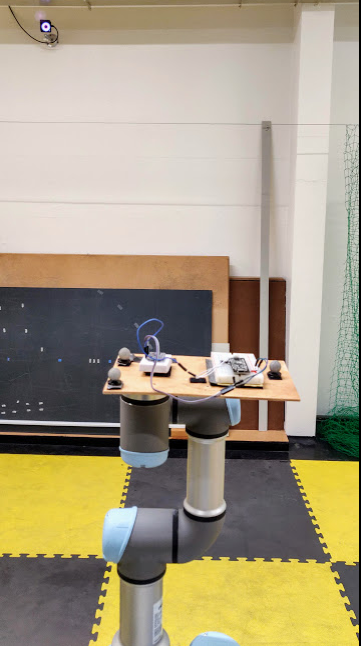
\includegraphics[scale=0.5]{graphics/Navigation/UR_static.png}
    \caption{IMU testbed on UR3 and Optitrack motion capture}
     \label{fig:IMU testbed}
\end{figure} 


In order to evaluate filters performance, two experiments were conducted for each algorithm:

\textbf{Experiment 1}

The first experiment evaluates the drift over time of the gyroscope without motion. The testbed is maintained static for 10 minutes for each filter; the data from all filters has been resampled to 100 Hz. 
Based on the measurements, the algorithms are evaluated with respect to the root mean square error and standard deviation from the reference point, compared to the raw integrated gyro data. 
The objective of this experiment is to compare the drift over time of the raw gyro measurements with the performance of the filters and selecting the algorithm that best minimizes this effect. 

\begin{figure}[h!]
    \centering
    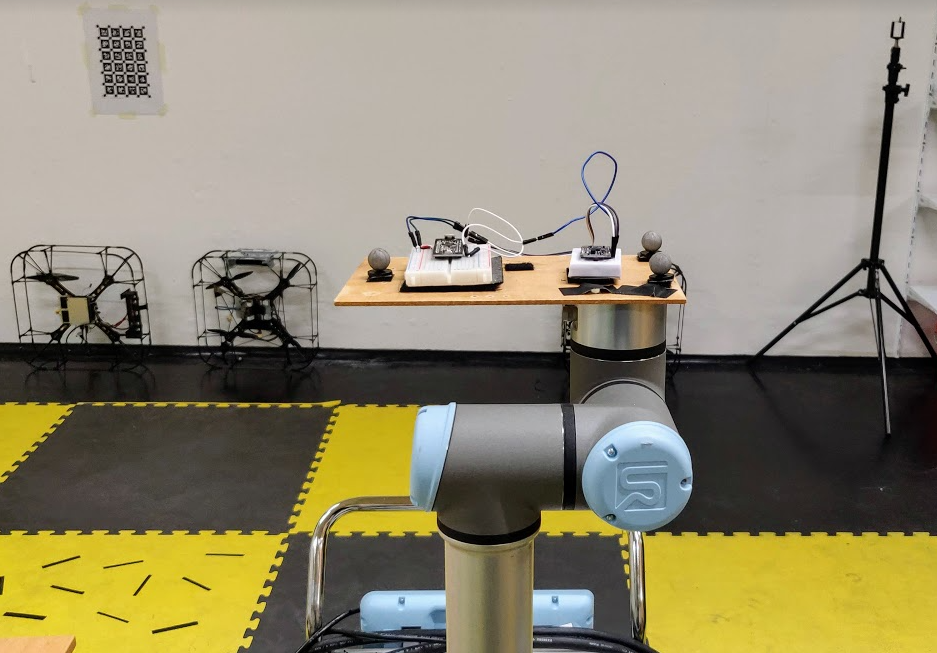
\includegraphics[scale=0.5]{graphics/Navigation/UR_2.png}
    \caption{IMU static testing}
     \label{fig:IMU static testing}
\end{figure} 


\textbf{Experiment 2}

The second experiment evaluates the performance of the filters in a motion ranging the IMU pitch angle from -45 to +45 degrees, involving all three components of the IMU in sensor fusion and comparing their performance against raw integrated gyro data and ground truth provided by the Optitrack motion capture system. The testbed performs three cycles of the full motion.
The objective of this experiment is to compare the performance of the filters against raw integrated gyro data and select the best performing algorithm in term of least deviation from the reference point from Optitrack. 

\begin{figure}[h!]
    \centering
    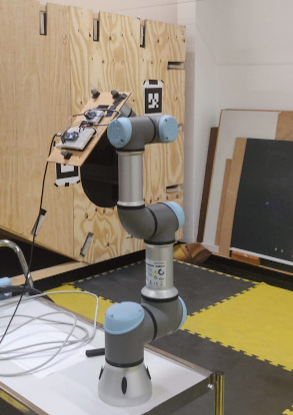
\includegraphics[scale=0.9]{graphics/Navigation/UR_inclined.png}
    \caption{IMU inclination testing}
     \label{fig:IMU inclination testing}
\end{figure} 


\subsection{Analysis of navigation performance}

Optitrack, Complementary filter and integrated gyro provide a relative measurement of yaw from their initial point, considered 0.
Mahony and Madgwick filter calculate absolute heading as measured by the magnetometer, based on the Earth's magnetic North. 
Due to the objective of this test is to measure the drift while static, all filters have been aligned to the absolute yaw measurement provided by the former two filters - then measuring deviations while the sensor is maintained static. 

\textbf{Experiment 1: Static test for comparing drift over time}

\begin{figure}[H]
    \centering
    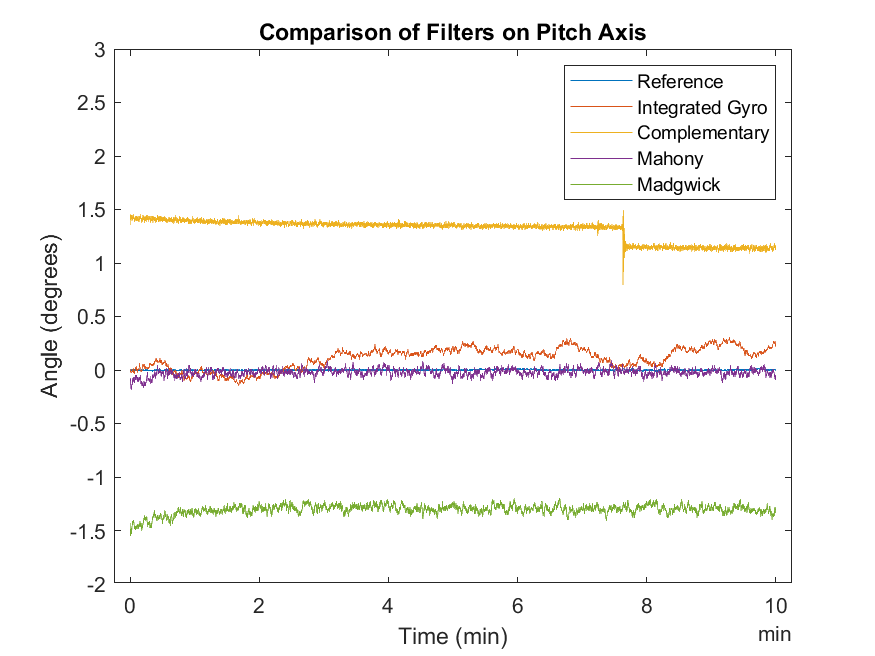
\includegraphics[scale=1]{graphics/Navigation/CombinedStaticPitch.png}
    \caption{Comparison of Filters on Pitch Axis}
     \label{fig:Comparison of Filters on Pitch Axis}
\end{figure} 

Figure \ref{fig:Comparison of Filters on Pitch Axis} compares the performance of the chosen fusion filters against the reference signal from Optitrack. Pitch axis has been selected because it coincides with the axis that the UAV can be tested on, with the current setup. Plots of the roll and yaw axes available in the appendix \ref{fig:Combined plot of roll axes for static test}, \ref{fig:Combined plot of yaw axes for static test}.

This is showing how each filter performs while static, to investigate the method that best minimizes drift over time and signal noise. 

The gyro is known to be better suited for motion rather than static applications, as it has low noise incidence but presents drift over time. 
The accelerometer is known to be stable over time, but has higher noise occurrences. In the case of the complementary filter in \ref{fig:IMU static testing}, the platform was not moved, therefore the most probable incident around 8:00 minute time that led to the spike was likely higher frequency accelerometer noise. This plot shows that the complementary filter does not compensate for such sudden spikes. The integrated gyro remained close to the reference 0 degrees for 3 minutes, after which an increase in drift is visible. Mahony filter performed best in this graph, closest to the reference point. The Madgwick filter shows steadiness in signal once converged, which seems to have taken about one minute with this beta parameter setting. The -1.3 offset is likely due to loss of calibration in the accelerometer and magnetometer data, showing it is more sensitive to this error than the Mahony filter. 

\begin{table}[H]
\centering
\begin{tabular}{ | m{7em} | m{1.5cm}|m{1.5cm}|m{1.5cm}|m{1.65cm}|m{1.5cm}|m{1.7cm}| } 
\hline
\textbf{Filters} & \textbf{Mean Roll }& \textbf{StdDev  Roll} & \textbf{Mean Pitch} &\textbf{ StdDev Pitch} & \textbf{Mean Yaw} & \textbf{ StdDev Yaw}  \\
\hline
\textit{Integrated Gyro} & -0.191 & 0.086 & 0.109 & 0.100& 197.02& 1.781 \\
\hline
\textit{Complementary Filter} & 0.478 &0.207 & 1.311 & 0.096&200.51 & 3.128 \\ 
\hline
\textit{Mahony Filter} & 0.086 &0.071 & -0.022 &0.033 &200.26 & 0.268 \\ 
\hline
\textit{Madgwick Filter} & 0.175 & 0.125 & -1.304 & 0.043 & 200.54 & 0.624\\
\hline
\end{tabular}
\caption{Table of navigation filters per axis for static test}
\label{table:1}
\end{table}

Table \ref{table:1} shows the performance of the filters for each separate axis. The mean value for roll and pitch is desired to be closer to 0, whereas for yaw it is desired to be closer to 200, the absolute yaw value as indicated by the sensor compass, while standard deviation is desired to be minimized. Based on these parameters, gyro integrated had a mean absolute offset of 0.1-0.2 degrees for roll and pitch and the largest yaw deviation of all filters. The other filters had similar yaw performance in static conditions. Complementary filter presented the largest roll and pitch offsets, as well as standard deviation overall. This is possibly due to the large weight given to gyro measurements in the filter, which tends to drift over time while static, possibly amplified by the incidence of accelerometer noise. It is expected that under movement, the adapting properties of the gyro will provide the filter with better performance. Mahony performed best both in terms of offset and noise, consistently across all axes. Madgwick measured slightly less well, unexpectedly, with a large deviation on pitch mean, but low noise; low roll offset but slightly higher noise than Mahony and gyro integrated and finally, good performance on yaw data. Madgwick is likely to have been more impacted  than Mahony by calibration errors. 


\textbf{Experiment 2: Motion test for comparing performance under movement}

\begin{figure}[H]
    \centering
    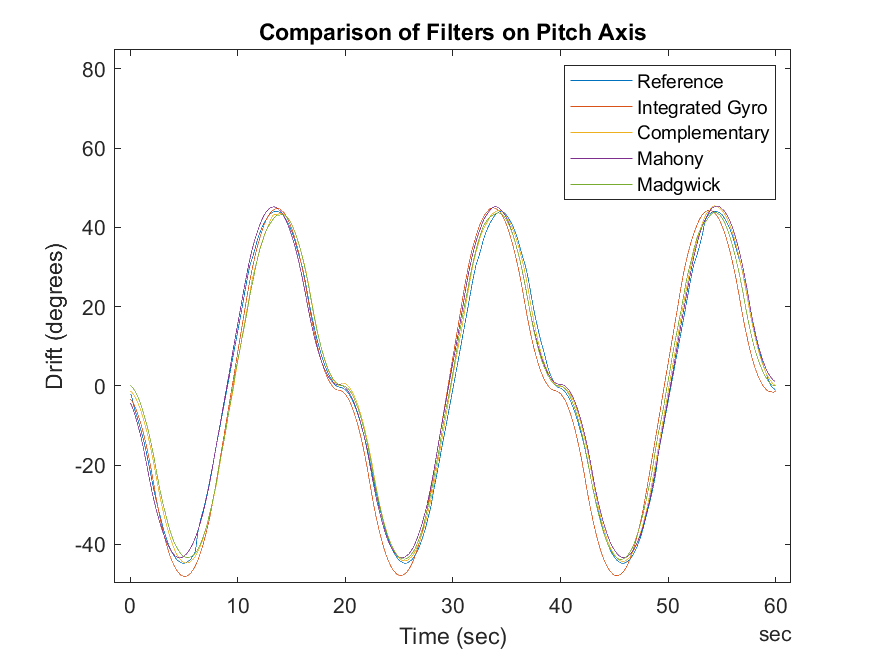
\includegraphics[scale=1]{graphics/Navigation/CombinedMotionPitch.png}
    \caption{Comparison of Filters on Pitch Axis in Motion}
     \label{fig:Comparison of Filters on Pitch Axis in Motion}
\end{figure} 

Figure \ref{fig:Comparison of Filters on Pitch Axis in Motion} compares the performance of the chosen fusion filters against the reference signal from Optitrack, during a motion of approximately +/- 45 degrees angle on the pitch axis. All filters performed well in motion, following the reference signal closely; the most significant being the deviation of 1.598 for the integrated gyro. However, on the roll (\ref{fig:Combined plot of roll axes for motion test}) and yaw (\ref{fig:Combined plot of yaw axes for motion test}) axes, some larger differences emerged. While it represented the trend of the motion well, the gyro shows a significant offset of 5.011 degrees from the reference. This is due to the fact that it lacks update from an absolute measurement, as the other filters do. It follows that integrating gyro is not reliable data on its own, due to not being able to detect the true angular position - but only the motion relative to its current (drifted) angle. This drift was particularly apparent on the yaw axis (\ref{fig:Combined plot of yaw axes for motion test}), where there is an upward drifting trend that does not follow reference well. The other outlier was complementary filter, having also challenges in following the motion reference on roll - and particularly so on yaw axis. The complementary filter is a suitable choice as far as roll and pitch is involved, but it is not reliable for yaw, as the deviation is too high compared to the other filters. Mahony had the smoothest and most accurate signal on roll but having flatter output on yaw than expected, with Madgwick having less smooth output on roll yet displaying a more reliable capture of the signal trend on yaw axis. 


\begin{table}[H]
\centering
\begin{tabular}{ | m{7em} | m{1.5cm}|m{1.5cm}|m{1.5cm}|m{1.5cm}|m{1.5cm}|m{1.5cm}| } 
\hline
\textbf{Filters} & \textbf{Mean Rol}l & \textbf{StdDev Roll}& \textbf{Mean Pitch} & \textbf{StdDev Pitch} & \textbf{Mean Yaw} &  \textbf{StdDev Yaw} \\
\hline
\textit{Integrated Gyro} & 5.011 & 1.657 & -1.598 & 30.641 &  178.86 & 0.770 \\
\hline
\textit{Complementary Filter}  & 0.995 & 1.445 & 0.041 & 29.496 &185.51 &  3.940 \\ 
\hline
\textit{Mahony Filter} & -0.060&1.805 & 0.575 & 29.547 &178.46 & 0.389 \\ 
\hline
\textit{Madgwick Filter}  &  -0.605 &0.652 & 0.026 & 28.882 & 181.3  &  1.124 \\
\hline
\end{tabular}
\caption{Table of navigation filters per axis for motion test}
\label{table:2}
\end{table}

The integrated gyro performs better in static than movement tests, in terms of both offset (mean) and noise measurement (std dev). While its yaw std.dev. is low, that measurement cannot be considered conclusive since it did not report well on the true motion. This difference between static and motion could potentially be accounted for by the additional drift from reference it experiences under movement, not having information about absolute measurements to correct this drift, thus leading to deviations wider in amplitude. The complementary filter encountered similar challenges, being 95 percent based on gyro measurements - it performed better in the static test. While its pitch and roll measurements were  fairly similar to Mahony and Madgwick filters, its yaw estimation is not usable, having widely deviated and provided particularly noisy output. Since it is a requirement in this project to have accurate yaw data, the integrated gyro and complementary filter prove to not be suitable. 

Mahony performed similarly to the static test, with reliable and consistent, measurements for both pitch and roll axis, with reliable signal trend capture. Yaw output was satisfactory, considering that the magnetometer lost and regained calibration during the motion, which impacted this measurement for both Mahony and Madgwick filters. It is expected that with more consistent sensor calibration, yaw output will improve. Madgwick filter also performed well - with best results on pitch axis  and best trend capture on yaw axis of all filters. Roll measurement was its most affected, but it still provided good data compared to integrated gyro and complementary - and overall a comparable performance to Mahony. 


\textbf{Combined measurements}

\begin{table}[h!]
\centering
\begin{tabular}{ | m{7em} | m{1.5cm}|m{1.75cm}| } 
\hline
\textbf{Filters} & \textbf{RMSE Static} & \textbf{RMSE Motion} \\
\hline
\textit{Integrated Gyro} & 3.4796 & 8.557   \\
\hline
\textit{Complementary Filter}&3.4712 & 8.057  \\ 
\hline
\textit{Mahony Filter} &0.3898& 3.3193  \\ 
\hline
\textit{Madgwick Filter}& 1.5579& 4.6223  \\
\hline
\end{tabular}
\caption{Table comparing RMSE performance of navigation filters}
\label{table:3}
\end{table}

The RMSE (Root Mean Squared Error) for each test was evaluated by taking the square root of the sum of squared differences between each filter axis and the reference (Optitrack). This metric was chosen because it provides an overview of each filter's deviation, combined across all axes. This deviation is in units of degrees, representing the offset compared to reference. 

Performance is measured by having a smaller RMSE value, closer to 0. 
The RMSE during the static tests show the iterative Mahony and Madgwick filters with a significantly improved performance over integrated gyro and complementary filters. This case holds for both static and motion tests.  The integrated gyro shows that indeed it is the least desirable option, with the complementary filter showing marginal improvement over it. 

During the tests, particularly during the motion test, calibration of the IMU was affected , especially so the accelerometer and magnetometer.
Therefore, filters Mahony and Madgwick relying on these two devices had their performance impacted more than the other two filters, relying on gyro only (integrated gyro) and accelerometer plus gyro (complementary filter). 

Even so, the two former iterative filters displayed improved performance and robustness over the integrated gyro and complementary. Mahony and Madgwick both suffered the same deterioration of calibration - out of which, Madgwick proved more sensitive to such impact, having a higher deviation (offset) as seen in the mean value per axis (absolute values of 0.175, 1.304, 0.624 for static test, and 0.026, 0.605, 18.7 for motion - compared to expected vales of 0 roll, 0 pitch, 200 yaw).

The calibration of the sensor is potentially affected by vibration of the robotic platform (linear acceleration read by the accelerometer), issues in initial calibration of the accelerometer, hard iron offsets due to the presence of metal surfaces in the robotic lab. Another point of impact on the performance of the filters is the hardware - the IMU is a low-cost device. 


\section{Experimental setup for control algorithm}


\subsection{Experimental setup - control test}

The objective is to test the controller on pitch axis, as designed, without interference from additional forces on the system. The initial setup had the drone oscillating wildly in its enclosure, therefore some changes were performed. 
The drone was reinforced with steel wire and adjusted into a rigid body, to remove side wobbling and products of inertia. 
In the previous setup, the propeller thrust was hitting the floor and influencing drone oscillations - therefore it was moved at a higher above floor level, hanged about its  center of mass and  restricted its motion to only allowing the pitch axis degree of freedom. 

It is outside of the scope of the project to control the thrust of the propellers - in the same manner that the rocket thrust is not handled by the guidance system, but given as a constant. 
Therefore, the testing is restricted to the drone's angular position, as influenced by the rudder deflecting the propeller thrust. Testing is performed with the drone tethered for safety, with its body frame placed at some inclination from its equilibrium point and measuring for the rise time, overshoot and settling time of the controller. 
The drone has been inclined to 0.2 to 0.8 absolute rotations in order to observe its response with different sets of gains.
Starting with a Proportional Gain of 2, as found by the simulation, the response has been as expected, with proportional response and overshoot.
Fig. \ref{fig:Controller with kP=2} shows the drone controller with kP=2, showing a fast response when inclined to 30 degrees, overshooting by 30 percent and with a settling time of 5 seconds. This response shows that a higher kP would not benefit the system, but only introduce more overshoot and longer settling time. 


\begin{figure}[H]
    \centering
    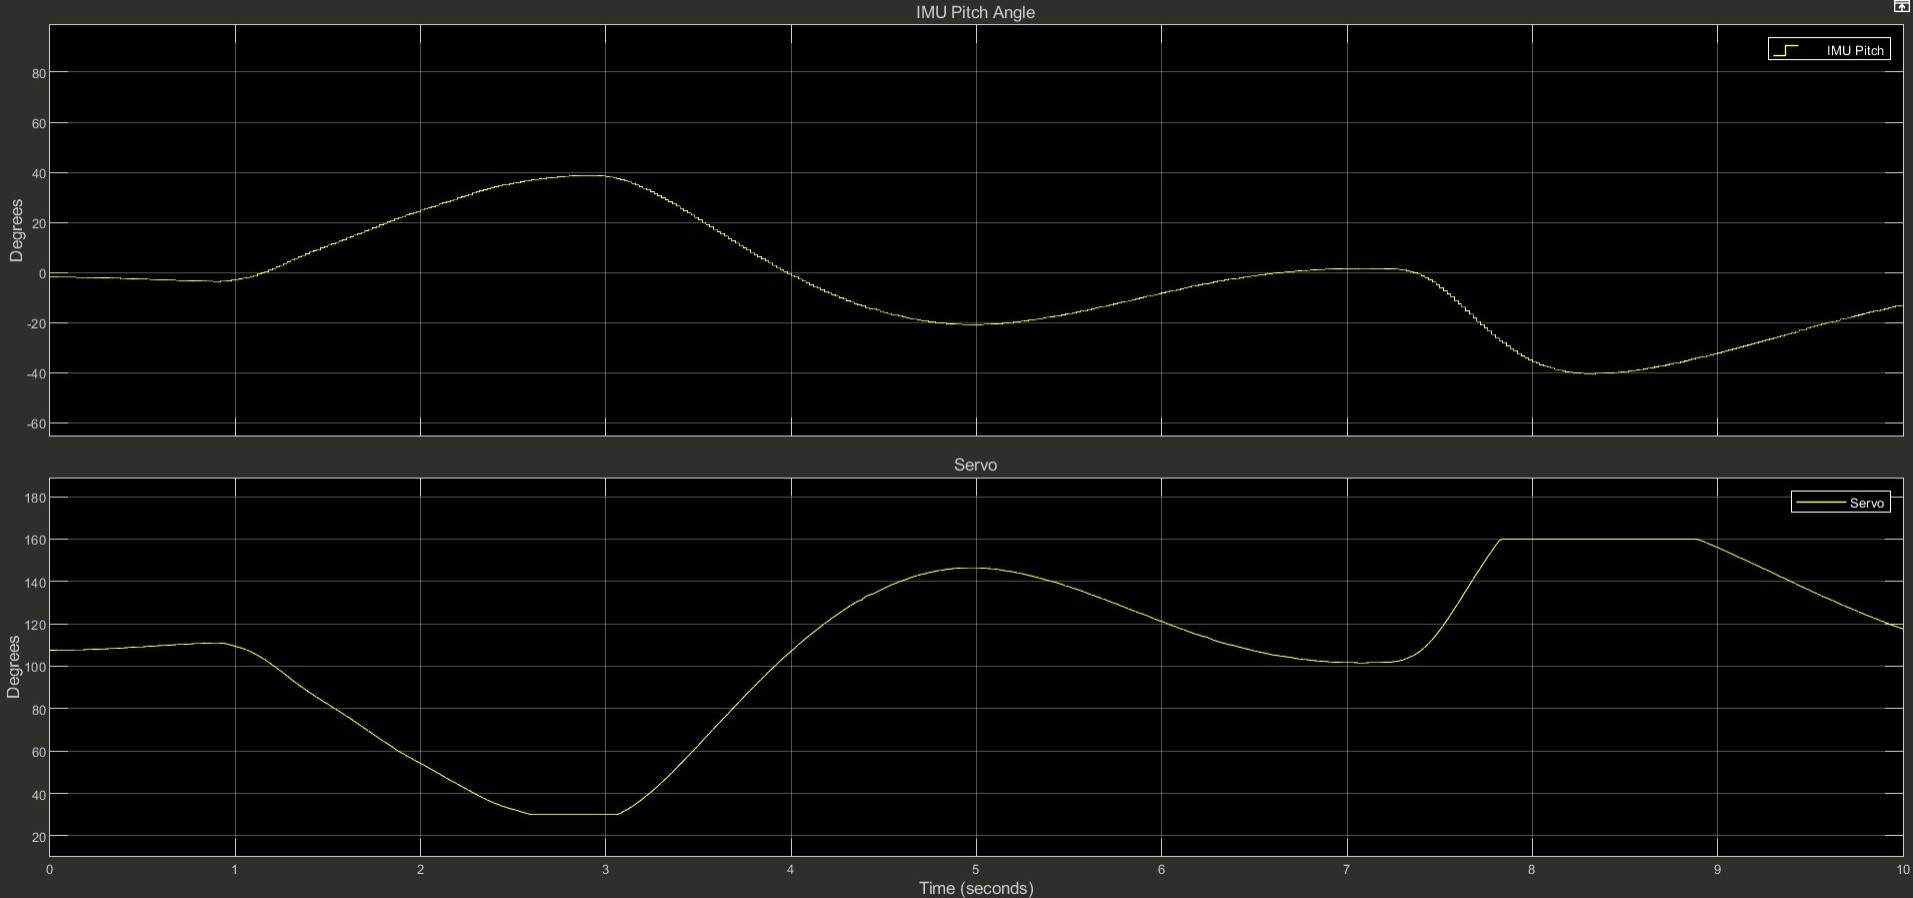
\includegraphics[scale=0.25]{graphics/Control/p2_Moment(2).jpg}
    \caption{Controller with kP=2}
     \label{fig:Controller with kP=2}
\end{figure} 

 Fig. \ref{fig:Controller with kP=2 kD=6} shows the controller with the set of gains kP=2, kD=6 found in the simulation. It was found that its response had too much jitter in servo movement and was not performing well. The jitter is most probably the result of the Derivative gain, which was an expected effect. However, the behavior observed was that the rudder would react with fast movements back and forth which were not adding to the performance. Instead, once the drone was brought to an inclination, rudder would move fast but then quickly resume its equilibrium position of 90 degrees, thus not influencing the drone position further but instead keeping it at the inclination it was manually brought to. 


\begin{figure}[H]
    \centering
    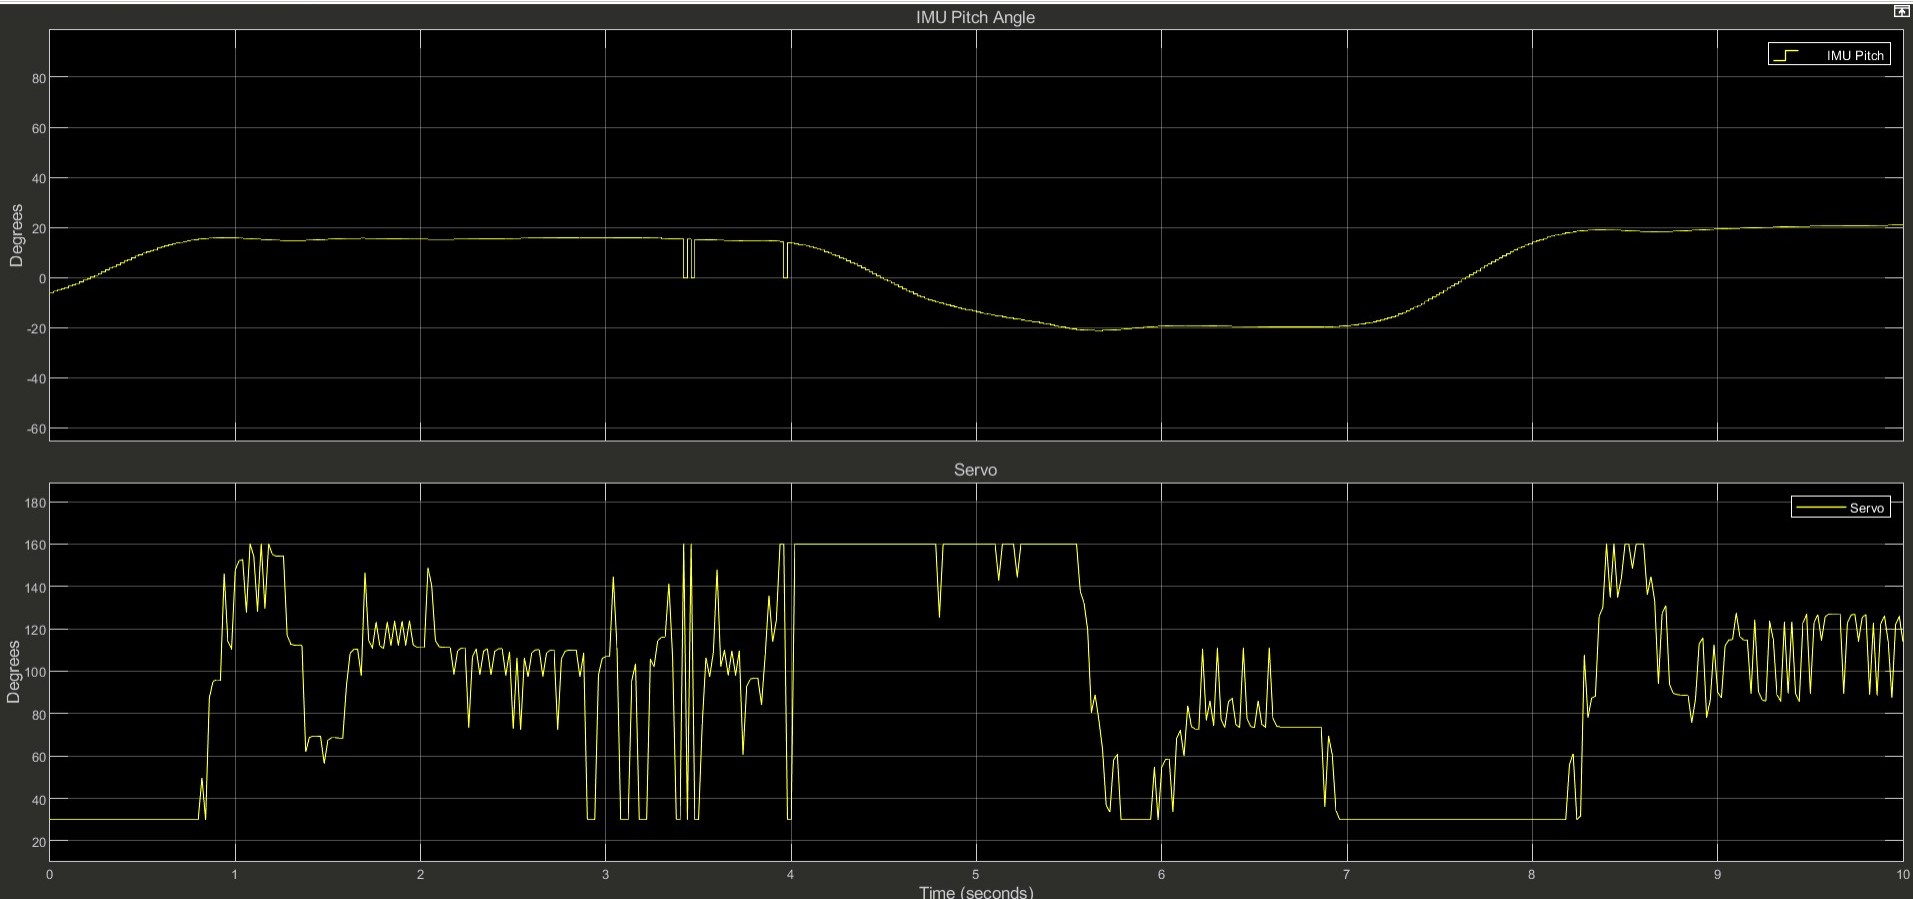
\includegraphics[scale=0.25]{graphics/Control/p2d6_Moment(3).jpg}
    \caption{Controller with kP=2 kD=6}
     \label{fig:Controller with kP=2 kD=6}
\end{figure} 

A controller with the same kP and a smaller kD=-0.1 has been however found to have no overshoot and a settling time of 2 seconds, so the Derivative gain has a positive effect on the performance. In fig. \ref{fig:Controller with kP=2 kD=-0.1}, the drone was first, manually inclined to 20 degrees at time t=2, and it reached equilibrium position at approx. t=3.8. The drone was inclined again, to the initial conditions specified in the Simulink model for the controller at approx. t=5.8, and it corrected itself to equilibrium 1.5 seconds later.

\begin{figure}[H]
    \centering
    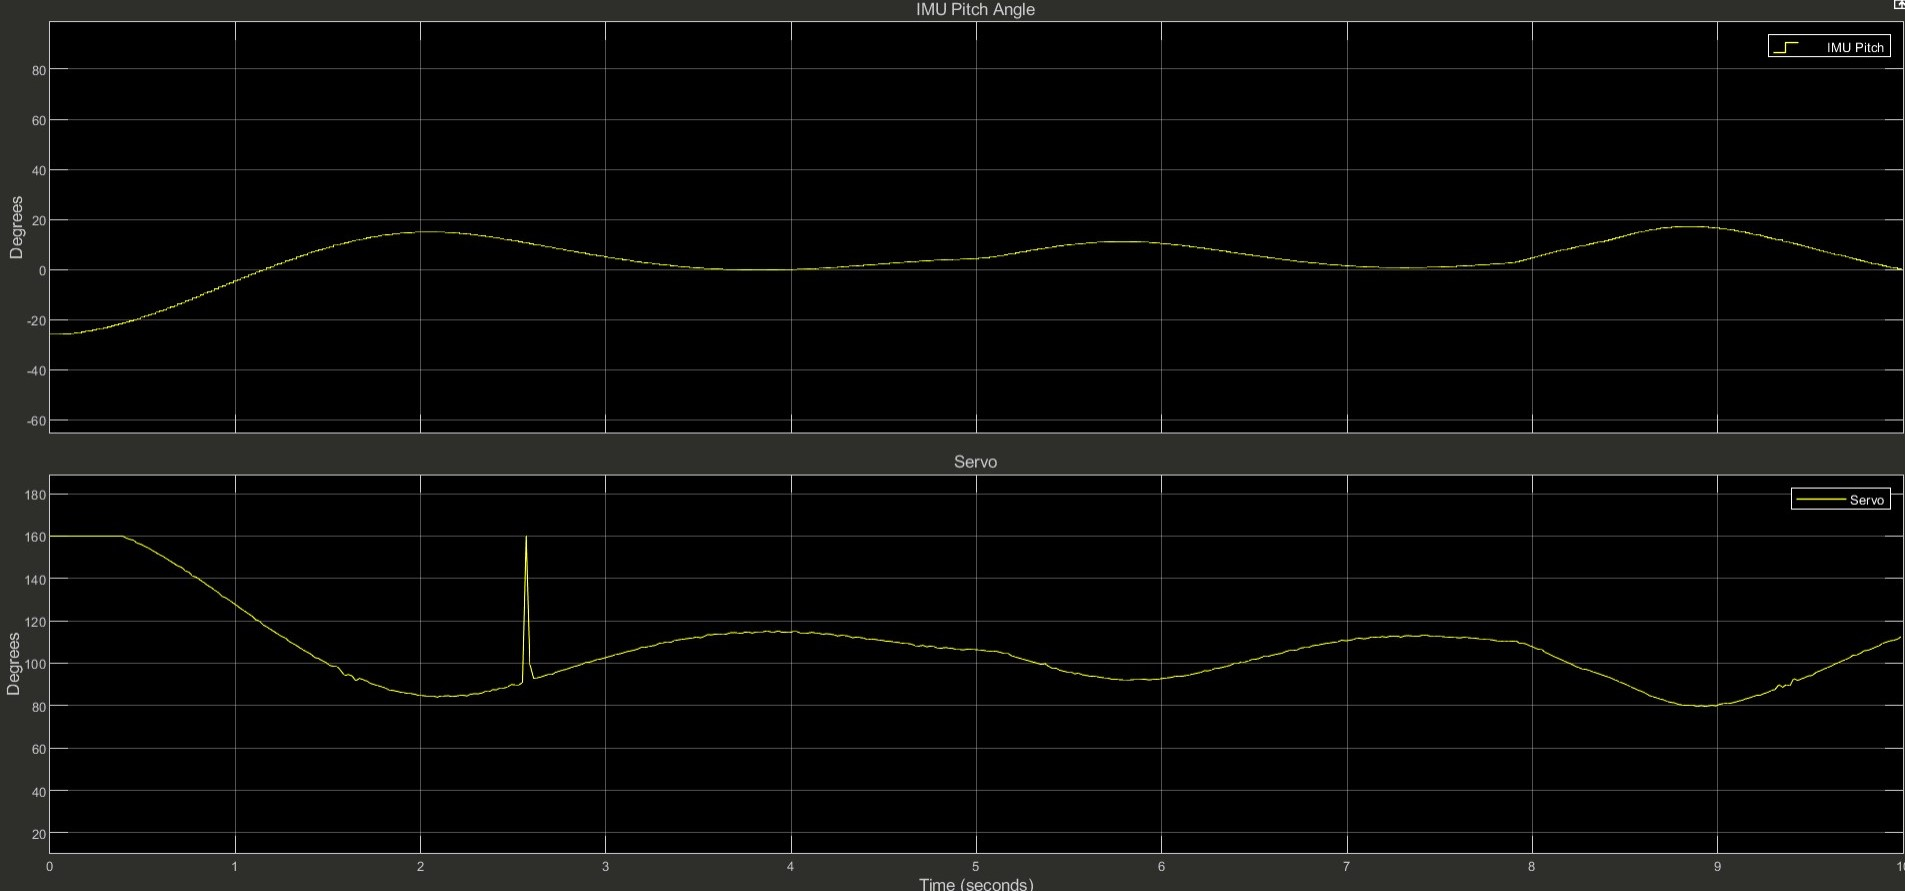
\includegraphics[scale=0.25]{graphics/Control/p2dminus01_Moment.jpg}
    \caption{Controller with kP=2 kD=-0.1}
     \label{fig:Controller with kP=2 kD=-0.1}
\end{figure} 

\subsection{Analysis of control performance}

Different tests of the controller behavior have been performed - it was found that a kP higher than the kP=2 based on the simulation was not beneficial and a lower value was too slow of a response. 
One potential reason why the response was slower than the simulation output is that the drone was not run at the thrust force value of 30N specified in the model. The propellers force is a function of input voltage and the battery supply was discharging fast during the tests, as the workshop had very low temperature. The drone was run on its lowest thrust value since the higher energy consumption would have lead to depleting the battery faster, thus possibly impeding further tests. 
The Derivative gain brings important performance improvements to the settling time of the system and minimizing overshoot. The value found in simulation is likely not realistic due to the amplification of response to navigation data noise. Smoother navigation signal would improve the output. Another possibility is, there might have been parameter deviations in the model. Further tests are needed to find a suitable kD parameter and improve the response time. 



This chapter demonstrated the use of the model-based control. Following, there will be the discussion of the results and the tests to be carried in future work. 
